\clearpage
\section{Walkthrough for Example 2}
\label{app-b}

This is the full walkthrough of the example in \autoref{overview:egraph-max} from the overview.

We walk through the steps needed to carry out the case splitting shown in \autoref{overview:egraph-max-min}.
The system contains the conditional rewrite rules shown on the right of \autoref{app-b:colored:example}, which 
constitute the definitions of $\tmax$ and $\tmin$,
plus some prior knowledge about $|\,{\cdot}\,|$ and $-$.

\newcolumntype{L}[1]{>{\raggedright\let\newline\\\arraybackslash\hspace{0pt}}m{#1}}

\begin{figure*}[t]
\begin{center}
\begin{tabular}{ll}
\begin{tabular}{L{3.5cm}l@{}}
    {\small (1)}\newline
    merge$\lowerred$($[x < y]$, $[\tfalse]$)
    &
    \raisebox{-0.5\totalheight}{\fbox{
      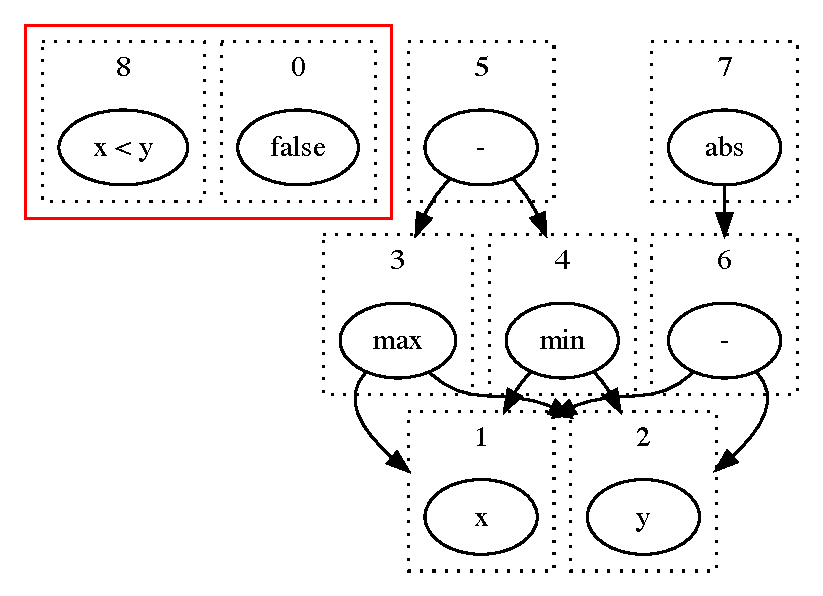
\includegraphics[width=4cm]{gfx/example_graphs_res/00-init.pdf}
    }}
    \\
    {\small (2)}\newline
    merge$\lowerred$($[\tmax(x, y)]$, $[x]$)\newline
    merge$\lowerred$($[\tmin(x, y)]$, $[y]$)\newline
    merge$\lowerred$($[|x - y|]$, $[x - y]$)
    &
    \raisebox{-0.5\totalheight}{\fbox{
      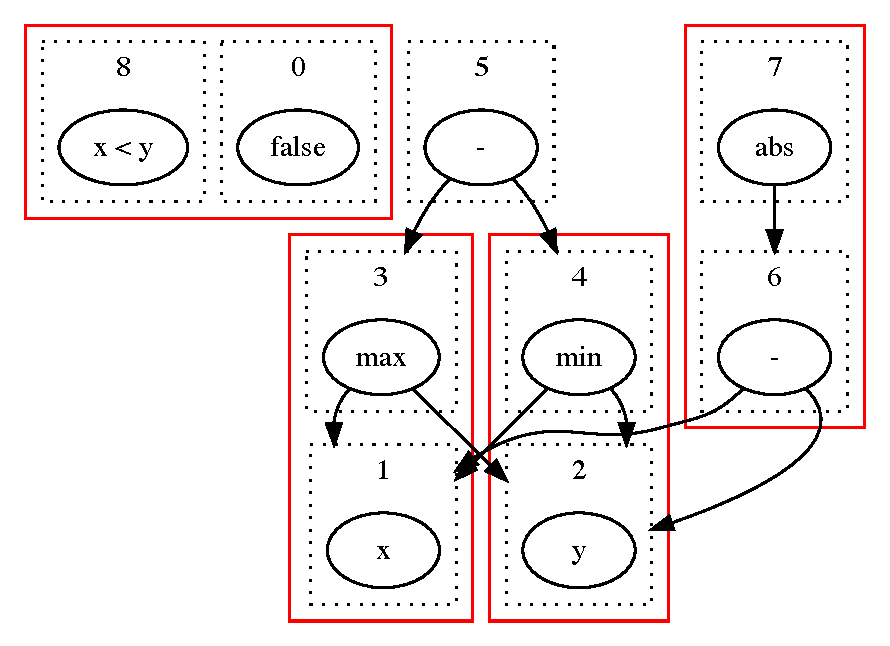
\includegraphics[width=4cm]{gfx/example_graphs_res/01-after_rw.pdf}
    }}  
    \\
    {\small (3)}\newline
    rebuild$\lowerred$() \newline
    \quad $\downarrow$ \newline
    merge$\lowerred$($[x - y]$, \newline
    \hspace{3em} $\tmax(x) - \tmin(y)$)
    &
    \raisebox{-0.5\totalheight}{\fbox{
    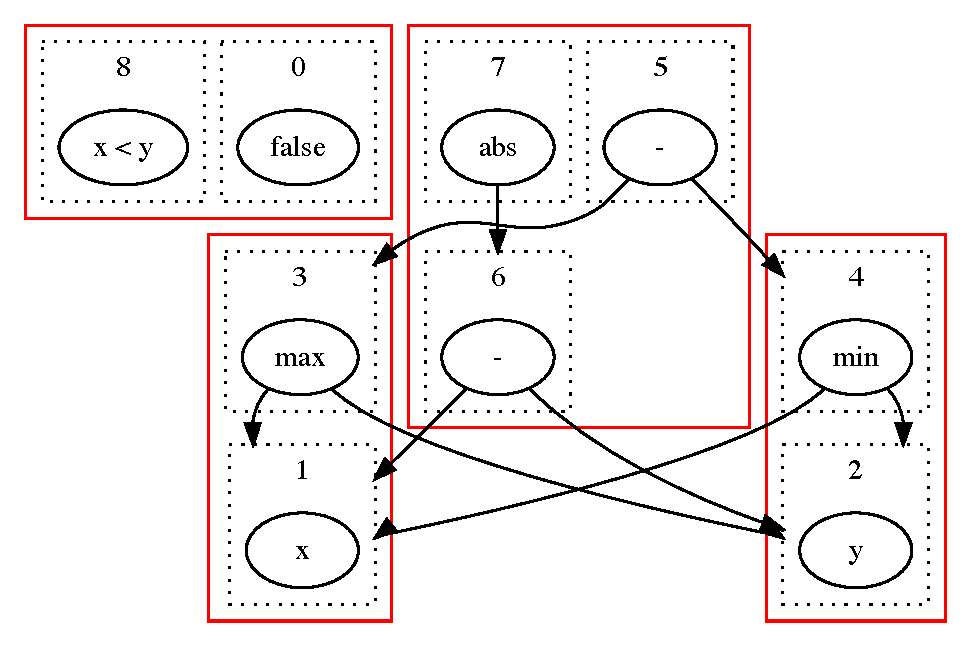
\includegraphics[width=4cm]{gfx/example_graphs_res/02-final.pdf}
    }}

\end{tabular}
%
&
\scalebox{0.9}{
$\begin{array}{c}
        \mbox{rewrite rules} \\ \arrayrulecolor{gray!50!white}\hline
        {?x} < {?y} \Rightarrow \tmin({?x}, {?y}) \rwto {?x} \\
        \lnot{?x} < {?y} \Rightarrow \tmin({?x}, {?y}) \rwto {?y} \\
        {?x} < {?y} \Rightarrow \tmax({?x}, {?y}) \rwto {?y} \\
        \lnot{?x} < {?y} \Rightarrow \tmax({?x}, {?y}) \rwto {?x} \\
        {?x} < {?y} \Rightarrow |{?x} - {?y}| \rwto {?y} - {?x} \\
        \lnot{?x} < {?y} \Rightarrow |{?x} - {?y}| \rwto {?x} - {?y} \\
    \end{array}$
}
\end{tabular}
%    
\caption{\label{app-b:colored:example}
    Rewriting with case-split in a colored e-graph.}

\end{center}
\end{figure*}

The semantics of a conditional rewrite rule in the domain of an e-graph is that the condition pattern should be matched and its root must be in the same e-class as $\ttrue$, and, additionally, the left-hand side should be matched as normal.
For simplicity of presentation, we pretend that $\lnot$ is a special case were the negated condition is e-matched and the e-class should contain $\tfalse$.

\smallskip
Starting with the base graph, \autoref{overview:egraph-max-min}(a), we describe the operation of Easter Egg
on the \cred color, corresponding to the case $\lnot x < y$.
The complement \cblue case ($x < y$) is analogous.

\begin{enumerate}[leftmargin=1.5em]
\item
    The value of $x < y$ is declared as $\tfalse$ via
    a colored merge.
    This yields a new \cred e-class.
\item
    Colored e-matching is performed against the premise of the c.r.r. $\lnot {?x} < {?y} \Rightarrow \tmax({?x}, {?y}) \rwto {?x}$.
    The condition of the rule, ${?x} < {?y}$, matches against the class $[x < y]$, 
    which is indeed in the same \cred e-class as $\tfalse$.
    
    Similar e-matches are carried out for the rules
    $\lnot {?x} < {?y} \Rightarrow \tmin({?x}, {?y}) \rwto {?y}$
    and
    $\lnot {?x} < {?y} \Rightarrow |{?x} - {?y}| \rwto {?x} - {?y}$.
\item
    The children of $\ecid3 - \ecid4 ~(\in M(\ecid5))$ are \cred-equivalent to those of $\ecid1 - \ecid2 ~(\in M(\ecid6))$, and,
    as a consequence, \cred congruence closure kicks in and performs a \cred union there.
\end{enumerate}

\medskip
The process for \cblue is analogous.
The case-split semantics is defined such that it records the fact
that \cblue and \cred are \emph{complements},
and as such extends $\equiv$ with the common equivalences,
$\congblue\cap\congred = \big\{\big\langle\ecid5,\ecid7\big\rangle, \ldots\big\}$.